%File principale del documento su cui invocare la compilazione, vedi "istruzioni.txt" per più info

%Preambolo: la parte prima del \begin{document}
\documentclass[12pt,a4paper]{article} %formato del documento e grandezza caratteri

%Input del file metadata.tex della cartella locale "res/"
%lista di comandi presenti in template_latex.tex, da qui posso essere modificati secondo le esigenze

\newcommand{\DocTitle}{Verbale interno 2019-11-18} %variabile usata dal file template_latex.tex per settare il titolo del documento
%\newcommand{\DocAuthor}{Progetto "Predire in Grafana"} %variabile usata dal file template_latex.tex per settare l'autore del documento
\newcommand{\DocDate}{18 Novembre 2019} %variabile usata dal file template_latex.tex; Impostata manualmente, altrimenti ad ogni compilazione viene messa la data del giorno di compilazione.
\newcommand{\DocDesc}{Resoconto dell'incontro del gruppo \textit{VRAM Software} tenutosi in data 2019-11-18} %variabile usata dal file template_latex.tex per settare la descrizione del documento
\newcommand{\ver}{27.0.0} %variabile usata dal file template_latex.tex per settare la versione del documento
\newcommand{\app}{Toffoletto Massimo} %variabile usata dal file template_latex.tex per settare l'approvatore del documento
\newcommand{\red}{Dalla Libera Marco} %variabile usata dal file template_latex.tex per settare il redattore del documento
\newcommand{\test}{Schiavon Rebecca} %variabile usata dal file template_latex.tex per settare il verificatore del documento
\newcommand{\stat}{Approvato} %variabile usata dal file template_latex.tex per settare lo stato del documento
\newcommand{\use}{Interno} %variabile usata dal file template_latex.tex per indicare l'uso del documento %Contiene le varibili che descrivono il documento

%Input di file di configurazione presi dalla cartella "Template-LaTeX/config/", uguali per tutti i documenti
%Attenzione bisogna impostare il percorso del file!
% Tutti i pacchetti usati, da inserire nel preambolo prima delle configurazioni

\usepackage[T1]{fontenc} %Permette la sillabazione su qualsiasi testo contenente caratteri
\usepackage[utf8]{inputenc} %Serve per usare la codifica utf-8
\usepackage[english,italian]{babel} %Imposta italiano lingua principale, inglese secondaria. Es. serve per far apparire "indice" al posto di "contents"

\usepackage{graphicx} %Serve per includere le immagini

\usepackage[hypertexnames=false]{hyperref} %Gestisce i riferimenti/link. Es. Serve per rendere clickabili le sezioni dell'indice

\usepackage{float} %Serve per migliore la definizione di oggetti fluttuanti come figure e tabelle. Es. poter usare l'opzione [H] nelle figure ovvero tenere fissate le immagini che altrimenti LaTeX si sposta a piacere.

\usepackage{listings} %Serve per poter mettere snippets di codice nel testo

\usepackage{lastpage} %Serve per poter introdurre un'etichetta a cui si può fare riferimento Es. piè di pagina; poter fare " \rfoot{\thepage\ di \pageref{LastPage}} "

\usepackage{fancyhdr} %Per header e piè di pagina personalizzati

%Sono alcuni package che potranno esserci utili in futuro
%\usepackage{charter}
%\usepackage{eurosym}
\usepackage{subcaption}
%\usepackage{wrapfig}
%\usepackage{background}
\usepackage{longtable} % tabella che può continuare per più di una pagina
\usepackage[table]{xcolor} % ho dovuto aggiungere table in modo da poter colorare le row della tabella, dava: undefined control sequences
%\usepackage{colortbl}

\usepackage{dirtree} % usato per creare strutte tree-view in stile filesystem
\usepackage{xspace} % usato per inserire caratteri spazio
\usepackage[official]{eurosym}
\usepackage{pdflscape} %Inclusione pacchetti
% Configurazioni varie, da inserire nel preambolo dopo i pacchetti

\hypersetup{hidelinks} %serve per nascondere riquadri rossi che circondano i link 

\lstset{literate= {à}{{\`a}}1 } %Permette di usare lettere accentate nei listings

\pagestyle{fancy} %Imposto stile pagina
\fancyhf{} %Reset, se lo tolgo LaTex mette impostazioni di default (p.es numerazione pagine di default)


\lhead{
\includegraphics[scale=0.25]{img/logo_header.png}} %Left header che compare in ogni pagina
%\rhead{\leftmark} %Nome della top-level structure (p.es. Section in article o Chapter in book) in ogni pagina
\rhead{\DocTitle\ v. \ver} %Right header

\newcommand{\glo}{$_G$} %Comando per aggiungere il pedice G
\newcommand{\glosp}{$_G$ } %Comando per aggiungere il pedice G con spazio

\newcommand\Tstrut{\rule{0pt}{2.6ex}} % top padding
\newcommand\Bstrut{\rule[-0.9ex]{0pt}{0pt}} % bottom padding
\newcommand{\TBstrut}{\Tstrut\Bstrut} % top & bottom padding

%Setto il colore dei link
%\hypersetup{
%	colorlinks,
%	linkcolor=[HTML]{404040},
%	citecolor={purple!50!black},
%	urlcolor={blue!50!black}
%}

%Tabelle e tabulazione (può tornare utile)
%\setlength{\tablcolsep}{10pt}
%\renewcommand{\arraystretch}{1.4}

%Comando per aggiungere le pagine di ogni sezione
%\newcommand{\newSection}[1]{%
%	\input{res/sections/#1}
%}

% Comandi per aggiungere padding a parole contenute nella tabella; è una specie di strut (un carattere invisibile)
%\newcommand\Tstrut{\rule{0pt}{2.6ex}} % top padding
%\newcommand\Bstrut{\rule[-0.9ex]{0pt}{0pt}} % bottom padding
%\newcommand{\TBstrut}{\Tstrut\Bstrut} % top & bottom padding 

\begin{document}
	%Input del file "frontmatter" preso dalla cartella "Template-LaTeX/config/", uguale per tutti i documenti
	%Attenzione bisogna impostare il percorso del file!
	%% #### FRONTESPIZIO (frontmatter) ####
\setlength{\headheight}{33pt} %Distanzia l'header
\pagenumbering{gobble} %Toglie il numero di pagina
\begin{titlepage}
	\begin{center}
		\vspace*{-2cm}
		
\includegraphics[scale=0.6]{img/logo.png} \\ %Logo
		\vspace{0.4cm} %Aggiunge uno spazio verticale di 0.5 cm
		
		{\LARGE Progetto "Predire in Grafana"} \\ %Nome progetto
		\vspace{0.4cm} %Attenzione a mettere il punto e NON la virgola
		
		{\Huge \textbf{\DocTitle}} \\ %Titolo, prende variabile definita in metadata.tex
		\vspace{0.4cm}
		
		\DocDate \\ %Data, prende variabile definita in metadata.tex
		\vspace{0.4cm}
		
		%Allineamento colonne: l=left r=right c=center, 
		%va specificato per ogni colonna
		%Se si vuole la riga tra colonne mettere "|"
		
		\begin{tabular}{r | l} %Elementi colonne separate da "&", le righe finiscono con "\\"
			Versione             & \ver \\
			Approvazione         & \app \\ 
			Redazione            & \red \\
			Verifica             & \test \\
			Stato                & \stat \\
			Uso                  & \use \\
		    Destinato a          & Zucchetti \\
						         & Prof. Vardanega Tullio\\
						         & Prof. Cardin Riccardo \\
			Email di riferimento & vram.software@gmail.com
		\end{tabular}
		\vfill
		\textbf{Descrizione} \\
		\DocDesc
	\end{center}
\end{titlepage}
\clearpage

% #### Impostazione header, footer  e numerazione pagine ####
\pagenumbering{arabic} %Pagine con i numeri arabi + reset a 1
\renewcommand{\footrulewidth}{0.4pt} %Di default footrulewidth==0 e quindi è invisibile, di default \headrulewith==0.4pt
\rfoot{\thepage\ di \pageref{LastPage}} %Pagina n di m, con numeri Arabi; usa il pacchetto "lastpage", in caso non sia possibile usare tale pacchetto mettere al fondo dell'ultima pagina "\label{LastPage}"

% #### Tabella dei log ####
% \textbf = grassetto; \Large = font più grande
% \rowcolors{quanti colori alternare}{colore numero riga pari}{colore numero riga dispari}: colori alternati per riga
% \rowcolor{color}: cambia colore di una riga
% p{larghezza colonna}: p è un tipo di colonna di testo verticalmente allineata sopra, ci sarebbe anche m che è centrata a metà ma non è precisa per questo utilizzo TBStrut; la sintassi >{\centering} indica che il contenuto della colonna dovrà essere centrato
% \TBstrut fa parte di alcuni comandi che ho inserito in config.tex che permetto di aggiungere un po' di padding al testo
% \\ [2mm] : questra scrittura indica che lo spazio dopo una break line deve essere di 2mm
% 

%\setcounter{secnumdepth}{0}
%\hfill \break
%\textbf{\Large{Diario delle modifiche}} \\


\addtocontents{toc}{\protect\setcounter{tocdepth}{0}} %Inserire questo per escludere una sezione dall'indice.

\section*{Registro delle modifiche} %Asterisco per fare sezione non numerata
\rowcolors{2}{gray!25}{gray!15}
\begin{longtable} {
		>{\centering}p{17mm} 
		>{\centering}p{19.5mm}
		>{\centering}p{24mm} 
		>{\centering}p{24mm} 
		>{}p{32mm}}
	\rowcolor{gray!50}
	\textbf{Versione} & \textbf{Data} & \textbf{Nominativo} & \textbf{Ruolo} & \textbf{Descrizione} \TBstrut \\
	14.7.0 & 2020-04-09 & Stantagiuliana Vittorio, Toffoletto Massimo e Spreafico Alessandro & \textit{Progettista}, \textit{Verificatore} e \textit{Responsabile di progetto} & Stesura, verifica e approvazione documento. \TBstrut \\ [2mm]
\end{longtable}

\addtocontents{toc}{\protect\setcounter{tocdepth}{4}} %Inserire questo per ripristinare il normale inserimento delle sezioni nell'indice. 4 significa fino al paragrah
\clearpage

% #### INDICE (tableofcontents) ####
\tableofcontents %Provoca la stampa dell'indice
\clearpage

\setcounter{secnumdepth}{4} %Permette di andare fino alla profondità del paragraph con la numerazione delle sezioni %Imposta il frontespizio, l'indice, header e footer
	
	
	
	%Tutte le sezioni del documento
	%\input{res/inserire nome sezione 1} 
	% ...
	%\input{res/inserire nome sezione n} 
	\section{Introduzione}
    \subsection{Scopo del documento}
        L'obiettivo di questo documento è riportare in modo puramente tecnico le scelte architetturali, strutturali e logiche intraprese dal gruppo \textit{VRAM Software} nel corso dello sviluppo del progetto \textit{Predire in Grafana}. Tale allegato sarà quindi corredato di vari diagrammi UML 2.x (classe, package e sequenza) che dimostreranno i vari design pattern adottati, la struttura del prodotto e i suoi scenari di esecuzione.
    \subsection{Scopo del prodotto}
        Il prodotto che il gruppo \textit{VRAM Software} sta approfondendo prevede lo sviluppo di un applicativo esterno e di un plug-in per la piattaforma di analisi Grafana\glosp per la predizione di dati tramite gli algoritmi di support vector machine (SVM) e di regressione lineare (RL). L'applicativo esterno fungerà da trainer generando un file JSON (predittore) partendo da dei dati in CSV a cui viene applicato l'algoritmo di predizione scelto dall'utente. Il file JSON ottenuto sarà poi inserito nel software Grafana tramite l'apposito plug-in e, dopo aver associato i nodi che si vogliono analizzare con i rispettivi predittori, sarà possibile visualizzare la previsione sul grafico della dashboard di Grafana. È inoltre presente la possibilità di salvare suddetti dati su un database InfluxDB. In tal modo il gruppo \textit{VRAM Software} insieme al proponente \textit{Zucchetti} punta ad agevolare l'attività di DevOps fornendo un valido strumento di predizione e monitoraggio dei dati.
    \subsection{Riferimenti}
        \subsubsection{Normativi}
            \begin{itemize}
                \item \textbf{Norme di Progetto}: \textit{Norme di Progetto v. 27.0.0};
                \item \textbf{Capitolato}\glosp \textbf{d'appalto}: \textit{C4 - Zucchetti - Predire in Grafana} \\
                 \url{https://www.math.unipd.it/~tullio/IS-1/2019/Progetto/C4.pdf}.
            \end{itemize}
        \subsection{Informativi}
        \begin{itemize}
        	\item \textbf{Analisi dei Requisiti}: \textit{Analisi dei Requisiti v. 27.0.0}
        \end{itemize}
        \subsection{Tecnici}
            \begin{itemize}
                \item \textbf{TypeScript}: \url{https://www.typescriptlang.org/docs/home.html};
                \item \textbf{JavaScript}: \url{https://developer.mozilla.org/it/docs/Web/JavaScript};
                \item \textbf{AngularJS}: \url{https://docs.angularjs.org/api};
                \item \textbf{React}: \url{https://it.reactjs.org/docs}.
            \end{itemize}
	\section*{Requisiti qualitativi}
	\rowcolors{2}{gray!25}{gray!15}
	\begin{longtable} {
		>{\centering}p{24mm} 
		>{\centering}p{32mm}
		>{\centering}p{40mm} 
		>{}p{24.5mm}
		}
	\rowcolor{gray!50}
		\textbf{Requisito} & \textbf{Classificazione} & \textbf{Descrizione} & \textbf{Fonti} 	\TBstrut \\
		R1Q1 & Obbligatorio & La documentazione e il codice dovranno rispettare le norme indicate nelle \textit{Norme di Progetto v. 1.1.1} e nel \textit{Piano di Qualifica v. 1.1.1} & Capitolato \TBstrut \\ [2mm]
		R1Q2 & Obbligatorio & Lo sviluppo del codice dovrà seguire le indicazioni date dallo strumento di analisi statica del codice SonarJS\glo & Interno \TBstrut \\ [2mm]
		R1Q3 & Obbligatorio & Deve essere stilato un manuale utente & Capitolato \TBstrut \\ [2mm]
        R1Q4 & Obbligatorio & Deve essere stilato un manuale manutentore & Capitolato \TBstrut \\ [2mm]
        R1Q5 & Obbligatorio & Il codice dovrà essere rilasciato con licenza Apache 2\glo & Capitolato \TBstrut \\ [2mm]
		R2Q6 & Desiderabile & Il codice e la documentazione dovranno essere versionati attraverso una repository\glosp GitHub & Capitolato \TBstrut \\ [2mm]
		R1Q7 & Obbligatorio & La documentazione sarà redatta in lingua italiana & Interno \TBstrut \\ [2mm]
	\end{longtable}
	\subsection{Requisiti di vincolo}
	\rowcolors{2}{gray!25}{gray!15}
	\begin{longtable} {
		>{\centering}p{18mm} 
		>{\centering}p{28mm}
		>{}p{50mm} 
		>{}p{28mm}
		}
	\rowcolor{gray!50}
	\textbf{Requisito} & 
	\textbf{Classificazione} & 
	\textbf{Descrizione} & 
	\textbf{Fonti} 	\TBstrut \\
	
	R1V1 & 
	Obbligatorio & 
	Il plug-in deve funzionare per l'ultima versione di Grafana\glo: \textit{6.5} &
	Interno  \TBstrut \\ [2mm]		
	
	R1V1.5 &
	Obbligatorio &
	Tutti i dati prodotti dovranno essere disponibili al sistema di Grafana\glosp per la creazione di grafici e dashboard\glo &
	Capitolato  \TBstrut \\ [2mm]
	
	R3V1.5.1 &
	Opzionale &
	Tutti i dati prodotti dal plug-in di Grafana\glosp dovranno essere disponibili al sistema stesso per la creazione di grafici e dashboard\glo &
	Interno  \TBstrut \\ [2mm]
	
	R1V1.5.2 &
	Obbligatorio &
	Tutti i dati prodotti dall'applicazione esterna per l'addestramento degli algoritmi di predizione dovranno essere disponibili al sistema di Grafana\glosp per la creazione di grafici e dashboard\glo &
	Interno  \TBstrut \\ [2mm]

	R1V2 & 
	Obbligatorio & 
	Il plug-in deve essere sviluppato attraverso tecnologie web &
	Capitolato  \TBstrut \\ [2mm]
	
	R1V2.1 & 
	Obbligatorio & 
	Il linguaggio di programmazione per il plug-in di Grafana\glosp deve essere Typescript &
	Interno  \TBstrut \\ [2mm]
	
	R1V2.2 & 
	Obbligatorio & 
	Il sistema deve funzionare sui browser più recenti dato il supporto dello standard ES6 &
	Interno  \TBstrut \\ [2mm]
	
	R1V2.2.1 & 
	Obbligatorio & 
	Il plug-in funziona sul browser Chrome dalla versione 58 in poi &
	Interno  \TBstrut \\ [2mm]
	
	R1V2.2.2 & 
	Obbligatorio & 
	Il plug-in funziona sul browser Microsoft Edge dalla versione 14 in poi &
	Interno  \TBstrut \\ [2mm]
	
	R1V2.2.3 & 
	Obbligatorio & 
	Il plug-in funziona sul browser Firefox dalla versione 54 in poi &
	Interno  \TBstrut \\ [2mm]
	
	R1V2.2.4 & 
	Obbligatorio & 
	Il plug-in funziona sul browser Safari dalla versione 10 in poi &
	Interno  \TBstrut \\ [2mm]
	
	R1V2.2.5 & 
	Obbligatorio & 
	Il plug-in funziona sul browser Opera dalla versione 55 in poi &
	Interno  \TBstrut \\ [2mm]
	
	R1V2.3 & 
	Obbligatorio & 
	Il plug-in deve utilizzare un build system\glosp che supporti systemjs, un caricatore di moduli ES (ECMAScript) &
	Interno  \TBstrut \\ [2mm]
	
	R2V2.5 &
	Desiderabile &
	La struttura dei file del plug-in deve essere simile alla struttura usata nella documentazione di Grafana\glo &
	Interno  \TBstrut \\ [2mm]
	
	R1V4 & 
	Obbligatorio & 
	L'applicazione esterna deve essere sviluppata attraverso tecnologie web &
	Capitolato \TBstrut \\ [2mm]
	
	R1V4.1 & 
	Obbligatorio & 
	Il linguaggio di programmazione per l'applicazione esterna deve essere Javascript e deve utilizzare lo standard \textit{ECMAScript6} (\textit{ES6}) &
	Interno  \TBstrut \\ [2mm]
	
	R1V4.2 & 
	Obbligatorio & 
	Il linguaggio di markup per l'applicazione esterna deve essere HTML5 e deve seguire lo standard W3C &
	Interno  \TBstrut \\ [2mm]
	
	R1V4.3 & 
	Obbligatorio & 
	Il linguaggio di presentazione per l'applicazione esterna deve essere CSS3 e deve seguire lo standard W3C &
	Interno  \TBstrut \\ [2mm]

	R1V4.4 & 
	Obbligatorio & 
	L'interfaccia utente dell'applicazione esterna deve essere sviluppata tramite il framework Javascript: React &
	Interno  \TBstrut \\ [2mm]

	R1V4.5 & 
	Obbligatorio & 
	La logica dell'applicazione, quindi l'interazione tra il sistema operativo e l'applicazione, deve essere sviluppata mediante codice NodeJs &
	Interno  \TBstrut \\ [2mm]

	R1V4.6 & 
	Obbligatorio & 
	Per sviluppare l'applicazione esterna deve essere utilizzato il framework Javascript Electron per gestire il rendering e la logica del prodotto &
	Interno  \TBstrut \\ [2mm]
	
	R1V5 & 
	Obbligatorio & 
	L'applicazione esterna deve funzionare nei sistemi operativi più recenti data la caratteristica di Electron di essere multipiattaforma & 
	Interno  \TBstrut \\ [2mm]

	R1V5.1 & 
	Obbligatorio & 
	L'applicazione esterna deve funzionare per il sistema operativo: Windows 10 &
	Interno  \TBstrut \\ [2mm]

	R1V5.2 & 
	Obbligatorio & 
	L'applicazione esterna deve funzionare per una qualsiasi distribuzione recente di Linux &
	Interno  \TBstrut \\ [2mm]

	R1V5.3 & 
	Obbligatorio & 
	L'applicazione esterna deve funzionare per il sistema operativo: MacOS Catalina &
	Interno  \TBstrut \\ [2mm]

	%MARCO R.
	%PROSEGUIRE SEGUENDO IL REQUISITO DI VINCOLO v2 E AGGIUNGENDO LE COSE CORRISPONDENTI CHE MANCANO
	%ESEMPIO: NELL'APP NON DEVE FUNZIONARE SUI BROWSER MA TRAMITE NODEJS + ELECTRON + REACT E QUINDI AGGIUGERE QUELLA COSA Lì ECC ECC
		
	R2V3 &
	Desiderabile &
	Il codice sorgente deve essere gestito mediante un sistema di versionamento\glosp (Git) e di Continuous Integration (GitHub Actions) &
	Interno  \TBstrut \\ [2mm]		
	
	R2V3.1 &
	Desiderabile &
	Il codice sorgente deve essere analizzato staticamente mediante SonarJs\glo &
	Interno  \TBstrut \\ [2mm]
	
	R2V3.2 &
	Desiderabile &
	Il codice sorgente deve essere analizzato dinamicamente mediante GitHub Actions e JS Unit Testing &
	Interno  \TBstrut \\ [2mm]
	
	R2V3.3 &
	Desiderabile &
	Devono essere eseguiti test funzionali mediante il framework: Selenium &
	Interno  \TBstrut \\ [2mm]
	
	%MARCO DALLAS
	%AGGIUNGERE EVENTUALMENTE DEI DETTAGLI SUI VINCOLI NELL'UTILIZZO DI GIT IN GENERALE
	\rowcolor{white}
	\caption{Requisiti vincolo}
\end{longtable}

	\section{Tracciamento}
    \subsection{Tracciamento requisiti funzionali}
        \rowcolors{2}{gray!25}{gray!15}
        \begin{longtable} {
            >{\centering}p{64.5mm} 
            >{}p{64.5mm}
            }
        \rowcolor{gray!50}
            \textbf{Requisito} & \textbf{Implementazione} \TBstrut \\
            R3F1 & Non implementato \TBstrut \\ [2mm]
            R3F1.1 & Non implementato \TBstrut \\ [2mm]
            R3F1.1.1 & Non implementato \TBstrut \\ [2mm]
            R3F1.1.2 & Non implementato \TBstrut \\ [2mm]
            R3F1.5 & Non implementato \TBstrut \\ [2mm]
            R3F1.6 & Non implementato \TBstrut \\ [2mm]
            R3F1.6.1 & Non implementato \TBstrut \\ [2mm]
            R3F1.6.2 & Non implementato \TBstrut \\ [2mm]
            R3F1.7 & Non implementato \TBstrut \\ [2mm]
            R3F1.2 & Non implementato \TBstrut \\ [2mm]
            R3F1.9 & Non implementato \TBstrut \\ [2mm]
            R3F1.10 & Non implementato \TBstrut \\ [2mm]
            R3F1.11 & Non implementato \TBstrut \\ [2mm]
            R3F1.12 & Non implementato \TBstrut \\ [2mm]
            R3F1.13 & Non implementato \TBstrut \\ [2mm]
            R3F1.14 & Non implementato \TBstrut \\ [2mm]
            R3F1.3 & Non implementato \TBstrut \\ [2mm]
            R3F1.4 & Non implementato \TBstrut \\ [2mm]
            R3F1.8 & Non implementato \TBstrut \\ [2mm]		
            R3F2 & Non implementato \TBstrut \\ [2mm]
            R3F2.1 & Non implementato \TBstrut \\ [2mm]
            R3F2.2 & Non implementato \TBstrut \\ [2mm]
            R3F2.3 & Non implementato \TBstrut \\ [2mm]
            R3F3 & Non implementato \TBstrut \\ [2mm]
            R3F17 & Non implementato \TBstrut \\ [2mm]	
            R1F4 & Implementato \TBstrut \\ [2mm]		
            R1F4.1 & Implementato \TBstrut \\ [2mm]		
            R1F4.1.1 & Implementato \TBstrut \\ [2mm]
            R1F4.1.2 & Implementato \TBstrut \\ [2mm]
            R1F4.8 & Implementato \TBstrut \\ [2mm]
            R1F4.9 & Implementato \TBstrut \\ [2mm]
            R1F4.9.1 & Implementato \TBstrut \\ [2mm]
            R1F4.9.2 & Implementato \TBstrut \\ [2mm]
            R1F4.10 & Implementato \TBstrut \\ [2mm]	
            R1F4.2 & Implementato \TBstrut \\ [2mm]
            R1F4.11 & Implementato \TBstrut \\ [2mm]
            R1F4.12 & Implementato \TBstrut \\ [2mm]
            R3F4.13 & Non implementato \TBstrut \\ [2mm]
            R3F4.14 & Non implementato \TBstrut \\ [2mm]
            R3F4.15 & Non implementato \TBstrut \\ [2mm]
            R3F4.16 & Non implementato \TBstrut \\ [2mm]		
            R1F4.4 & Implementato \TBstrut \\ [2mm]
            R1F4.5 & Implementato \TBstrut \\ [2mm]		
            R2F4.6 & Implementato \TBstrut \\ [2mm]		
            R1F4.7 & Implementato \TBstrut \\ [2mm]
            R1F5 & Non implementato \TBstrut \\ [2mm]
            R1F5.1 & Non implementato \TBstrut \\ [2mm]
            R1F5.2 & Non implementato \TBstrut \\ [2mm]
            R1F5.3 & Non implementato \TBstrut \\ [2mm]
            R2F6 & Non implementato \TBstrut \\ [2mm]
            R2F18 & Non implementato \TBstrut \\ [2mm]
            R1F19 & Implementato \TBstrut \\ [2mm]
            R1F7 & Implementato \TBstrut \\ [2mm]
            R1F21 & Implementato \TBstrut \\ [2mm]
            R1F8 & Implementato \TBstrut \\ [2mm]
            R1F9 & Implementato \TBstrut \\ [2mm]
            R1F9.1 & Implementato \TBstrut \\ [2mm]
            R1F9.2 & Implementato \TBstrut \\ [2mm]
            R3F9.3 & Non implementato \TBstrut \\ [2mm]
            R1F9.4 & Implementato \TBstrut \\ [2mm]
            R2F9.5 & Implementato \TBstrut \\ [2mm]
            R2F10 & Non implementato \TBstrut \\ [2mm]
            R1F11 & Implementato \TBstrut \\ [2mm]
            R1F12 & Implementato \TBstrut \\ [2mm]	
            R1F20 & Implementato \TBstrut \\ [2mm]	
            R2F13 &	Non implementato \TBstrut \\ [2mm]					
            R2F13.2 & Non implementato \TBstrut \\ [2mm]		
            R2F13.3 & Non implementato \TBstrut \\ [2mm]
            R2F13.4 & Non implementato \TBstrut \\ [2mm]		
            R2F14 &	Non implementato \TBstrut \\ [2mm]
            R2F15 &	Non implementato \TBstrut \\ [2mm]		
            R2F16 & Non implementato \TBstrut \\ [2mm]
            \rowcolor{white}
            \caption{Tracciamento implementazione requisiti funzionali}
        \end{longtable}
        \begin{figure}[H]
            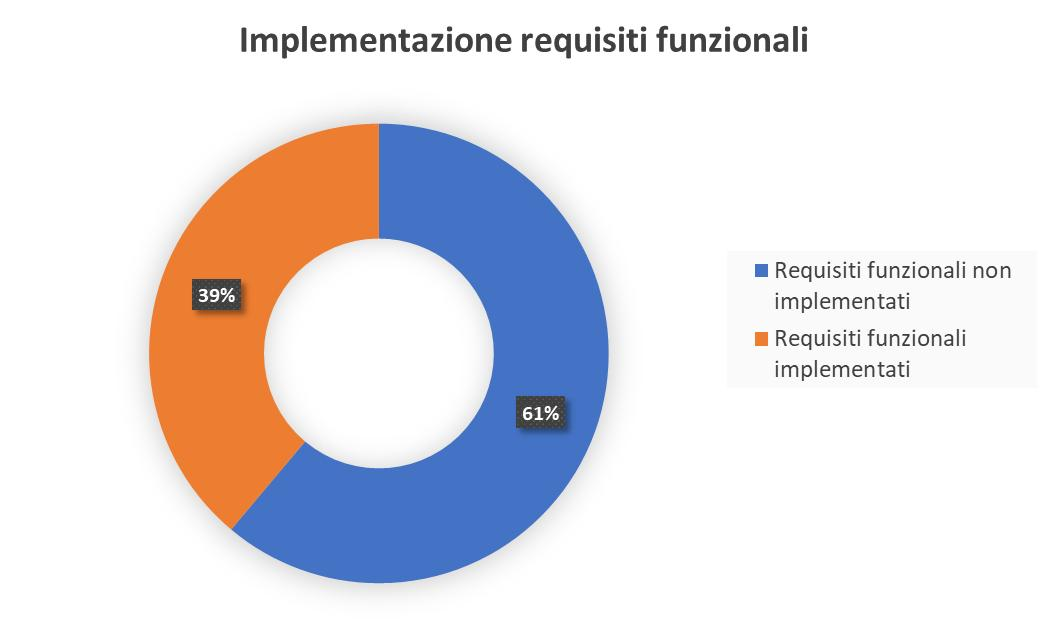
\includegraphics[width=\textwidth,height=\textheight,keepaspectratio]{./img/Grafici/implementazione_requisiti_funzionali.jpg}
            \caption{Grafico implementazione requisiti funzionali}
        \end{figure}
        \begin{figure}[H]
            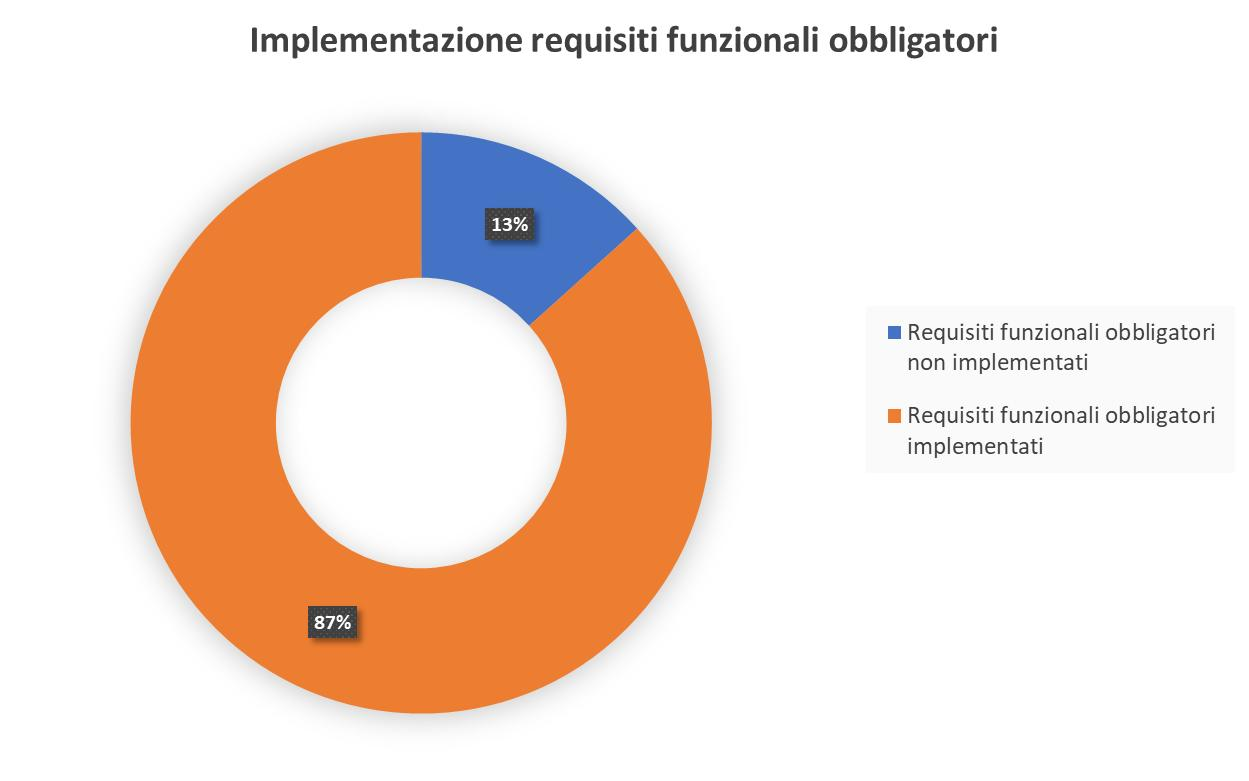
\includegraphics[width=\textwidth,height=\textheight,keepaspectratio]{./img/Grafici/implementazione_requisiti_funzionali_obbligatori.jpg}
            \caption{Grafico implementazione requisiti funzionali obbligatori}
        \end{figure}
    \subsection{Tracciamento requisiti qualitativi}
        \rowcolors{2}{gray!25}{gray!15}
        \begin{longtable} {
            >{\centering}p{64.5mm} 
            >{}p{64.5mm}
            }
        \rowcolor{gray!50}
            \textbf{Requisito} & \textbf{Implementazione} \TBstrut \\
            R1Q1 & Implementato \TBstrut \\ [2mm]
            R1Q2 & Implementato \TBstrut \\ [2mm]
            R1Q10 & Implementato \TBstrut \\ [2mm]
            R1Q3 & Implementato \TBstrut \\ [2mm]
            R1Q4 & Implementato \TBstrut \\ [2mm]
            R1Q5 & Implementato \TBstrut \\ [2mm]
            R2Q6 & Implementato \TBstrut \\ [2mm]
            R1Q7 & Implementato \TBstrut \\ [2mm]
            R1Q8 & Implementato \TBstrut \\ [2mm]
            R1Q9 & Implementato \TBstrut \\ [2mm]
            R1Q11 & Implementato \TBstrut \\ [2mm]
            \rowcolor{white}
            \caption{Tracciamento implementazione requisiti qualitativi}
        \end{longtable}
        \begin{figure}[H]
            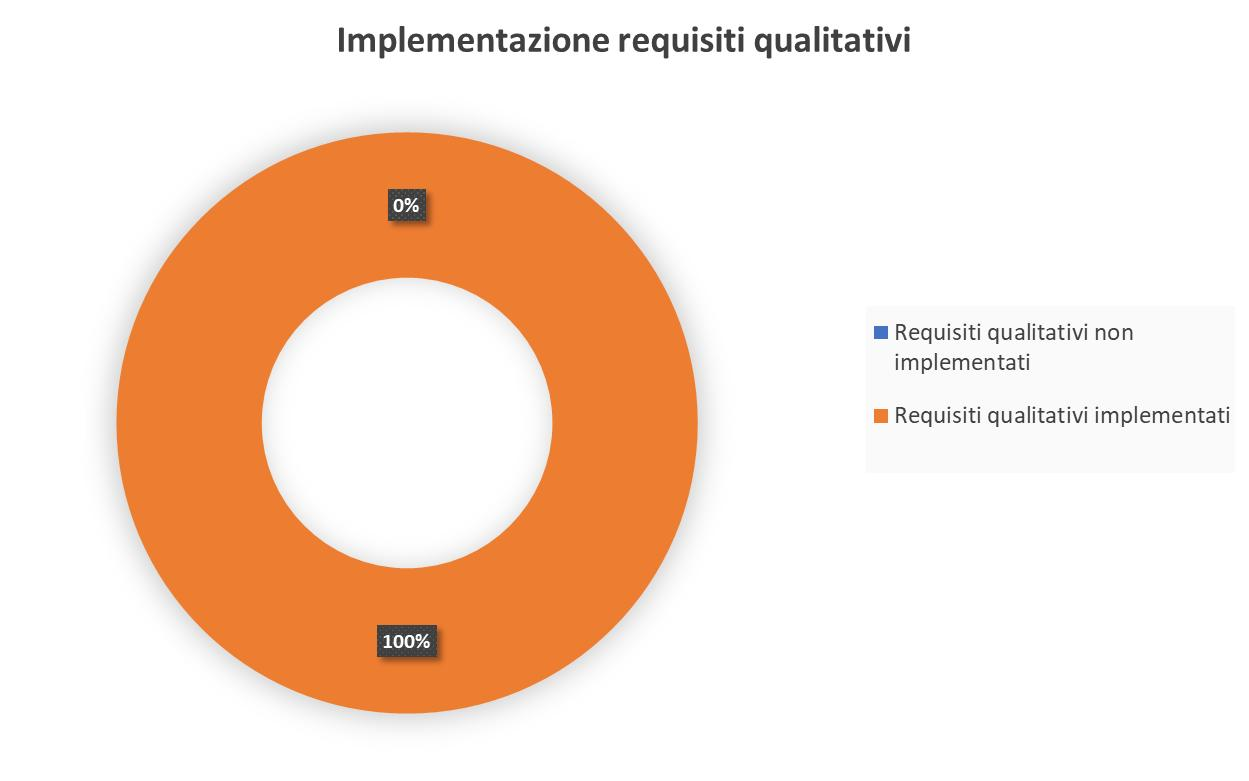
\includegraphics[width=\textwidth,height=\textheight,keepaspectratio]{./img/Grafici/implementazione_requisiti_qualitativi.jpg}
            \caption{Grafico implementazione requisiti qualitativi}
        \end{figure}
        \begin{figure}[H]
            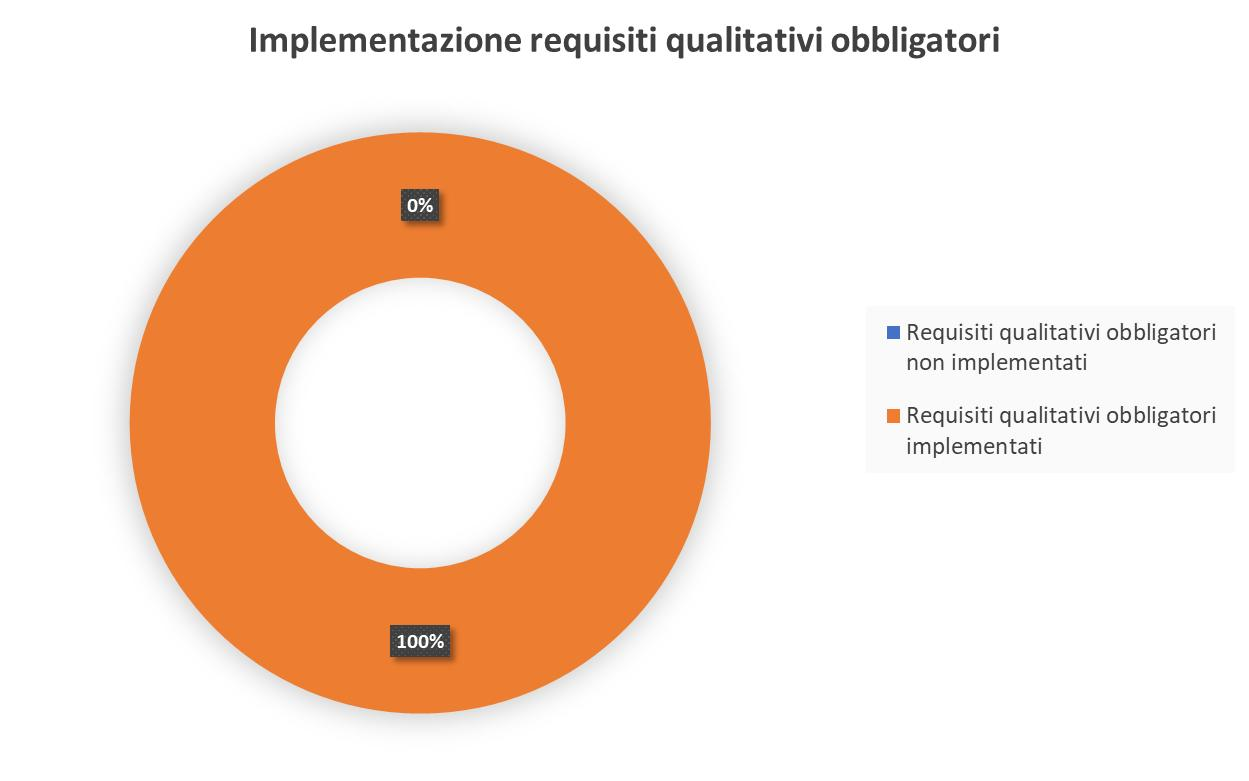
\includegraphics[width=\textwidth,height=\textheight,keepaspectratio]{./img/Grafici/implementazione_requisiti_qualitativi_obbligatori.jpg}
            \caption{Grafico implementazione requisiti qualitativi obbligatori}
        \end{figure}
    \subsection{Tracciamento casi d'uso}
        \rowcolors{2}{gray!25}{gray!15}
        \begin{longtable} {
            >{\centering}p{64.5mm} 
            >{}p{64.5mm}
            }
        \rowcolor{gray!50}
            \textbf{Caso d'uso} & \textbf{Implementazione} \TBstrut \\
            UC1 & Non implementato \TBstrut \\ [2mm]
            UC1.1 & Non implementato \TBstrut \\ [2mm]
            UC1.2 & Non implementato \TBstrut \\ [2mm]
            UC1.3 & Non implementato \TBstrut \\ [2mm]
            UC1.4 & Non implementato \TBstrut \\ [2mm]
            UC1.5 & Non implementato \TBstrut \\ [2mm]
            UC1.6 & Non implementato \TBstrut \\ [2mm]
            UC1.7 & Non implementato \TBstrut \\ [2mm]
            UC1.8 & Non implementato \TBstrut \\ [2mm]
            UC1.9 & Non implementato \TBstrut \\ [2mm]
            UC1.10 & Non implementato \TBstrut \\ [2mm]
            UC1.11 & Non implementato \TBstrut \\ [2mm]
            UC1.12 & Non implementato \TBstrut \\ [2mm]
            UC1.13 & Non implementato \TBstrut \\ [2mm]
            UC1.14 & Non implementato \TBstrut \\ [2mm]
            UC2 & Non implementato \TBstrut \\ [2mm]
            UC2.1 & Non implementato \TBstrut \\ [2mm]
            UC2.2 & Non implementato \TBstrut \\ [2mm]
            UC2.3 & Non implementato \TBstrut \\ [2mm]
            UC3 & Non implementato \TBstrut \\ [2mm]
            UC4 & Implementato \TBstrut \\ [2mm]
            UC4.1 & Implementato\TBstrut \\ [2mm]
            UC4.2 & Implementato \TBstrut \\ [2mm]
            UC4.3 & Implementato \TBstrut \\ [2mm]
            UC4.4 & Implementato \TBstrut \\ [2mm]
            UC4.5 & Implementato \TBstrut \\ [2mm]
            UC4.6 & Implementato \TBstrut \\ [2mm]
            UC4.7 & Implementato \TBstrut \\ [2mm]
            UC4.8 & Implementato \TBstrut \\ [2mm]
            UC4.9 & Implementato \TBstrut \\ [2mm]
            UC4.10 & Implementato \TBstrut \\ [2mm]
            UC4.11 & Implementato \TBstrut \\ [2mm]
            UC4.12 & Non implementato \TBstrut \\ [2mm]
            UC4.13 & Non implementato \TBstrut \\ [2mm]
            UC4.14 & Non implementato \TBstrut \\ [2mm]
            UC4.15 & Non implementato \TBstrut \\ [2mm]
            UC5 & Non implementato \TBstrut \\ [2mm]
            UC5.1 & Non implementato \TBstrut \\ [2mm]
            UC5.2 & Non implementato \TBstrut \\ [2mm]
            UC5.3 & Non implementato \TBstrut \\ [2mm]
            UC6 & Non implementato \TBstrut \\ [2mm]
            UC7 & Implementato \TBstrut \\ [2mm]
            UC8 & Implementato \TBstrut \\ [2mm]
            UC9 & Implementato \TBstrut \\ [2mm]
            UC9.1 & Implementato \TBstrut \\ [2mm]
            UC9.2 & Implementato \TBstrut \\ [2mm]
            UC9.3 & Implementato \TBstrut \\ [2mm]
            UC9.4 & Implementato \TBstrut \\ [2mm]
            UC10 & Non implementato \TBstrut \\ [2mm]
            UC12 & Implementato \TBstrut \\ [2mm]
            UC13 & Non implementato \TBstrut \\ [2mm]
            UC13.2 & Non implementato \TBstrut \\ [2mm]
            UC13.3 & Non implementato \TBstrut \\ [2mm]
            UC13.4 & Non implementato \TBstrut \\ [2mm]
            UC14 & Non implementato \TBstrut \\ [2mm]
            UC15 & Non implementato \TBstrut \\ [2mm]
            UC16 & Non implementato \TBstrut \\ [2mm]
            UC17 & Non implementato \TBstrut \\ [2mm]
            UC18 & Non implementato \TBstrut \\ [2mm]
            UC19 & Implementato \TBstrut \\ [2mm]
            UC20 & Implementato \TBstrut \\ [2mm]
            UC21 & Implementato \TBstrut \\ [2mm]
            \rowcolor{white}
            \caption{Tracciamento implementazione casi d'uso\glo}
        \end{longtable}
        \begin{figure}[H]
            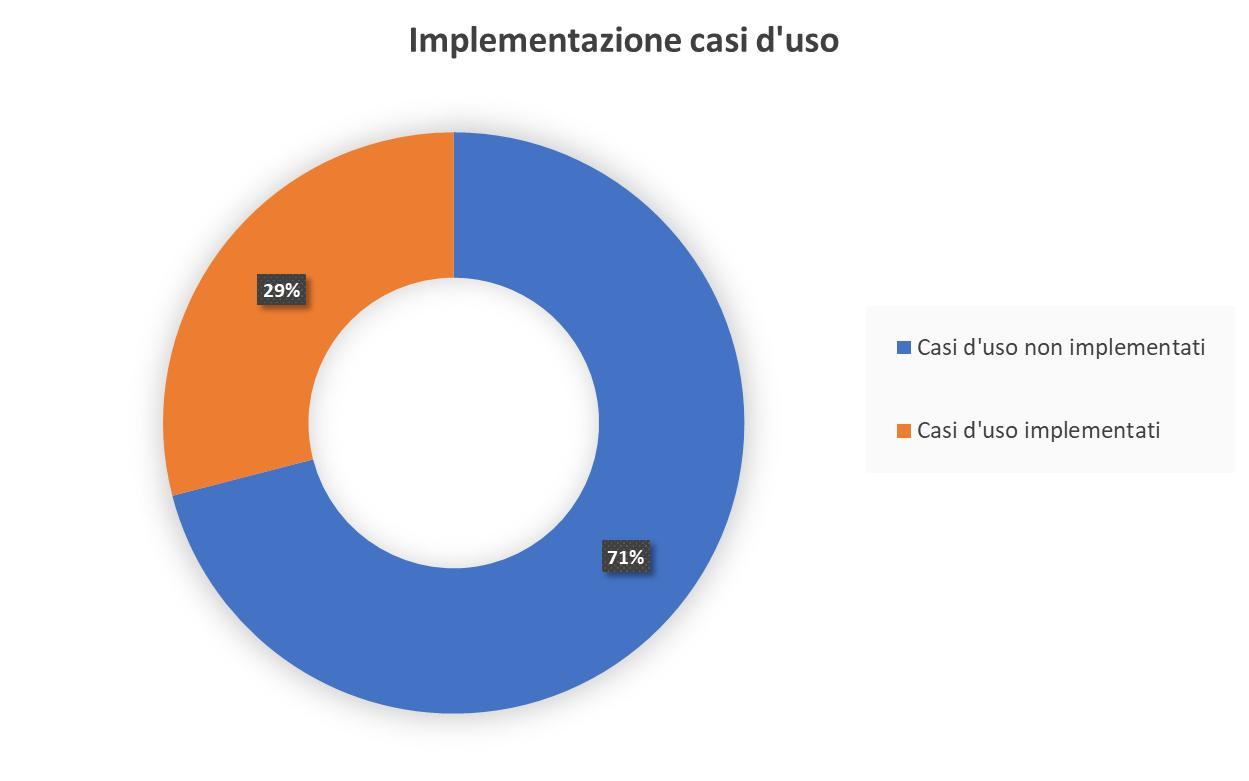
\includegraphics[width=\textwidth,height=\textheight,keepaspectratio]{./img/Grafici/implementazione_casi_d'uso.jpg}
            \caption{Grafico implementazione casi d'uso\glo}
        \end{figure}
	
	
	%Input del file "decision_table" della cartella locale "res/"
	%% \textbf = grassetto; \Large = font più grande
% \rowcolors{quanti colori alternare}{colore numero riga pari}{colore numero riga dispari}: colori alternati per riga
% \rowcolor{color}: cambia colore di una riga
% p{larghezza colonna}: p è un tipo di colonna di testo verticalmente allineata sopra, ci sarebbe anche m che è centrata a metà ma non è precisa per questo utilizzo TBStrut; la sintassi >{\centering} indica che il contenuto della colonna dovrà essere centrato
% \TBstrut fa parte di alcuni comandi che ho inserito in config.tex che permetto di aggiungere un po' di padding al testo
% \\ [2mm] : questra scrittura indica che lo spazio dopo una break line deve essere di 2mm

%\setcounter{secnumdepth}{0}
%\hfill \break
%\textbf{\Large{Diario delle modifiche}} \\
\section{Riepilogo tracciamenti}
\rowcolors{2}{gray!25}{gray!15}
\begin{longtable} {
		>{\centering}p{17mm} 
		%>{\centering}p{19.5mm}
		%>{\centering}p{24mm} 
		%>{\centering}p{24mm} 
		>{}p{120mm}}
	\rowcolor{gray!50}
	\textbf{Codice} & \multicolumn{1}{c}{\textbf{Decisione}} \\%\textbf{Decisione} \\ %\TBstrut \\
	VI\_2.1 & Divisione dei ruoli per inizio stesura documenti. \TBstrut \\ [2mm]
	VI\_2.2 & Studio preliminare e divisione del carico di lavoro per le \textit{Norme di Progetto v. 1.1.1} \TBstrut \\ [2mm]
	VI\_2.3 & Stesura domande per l'incontro con il proponente \textit{Zucchetti}. \TBstrut \\ [2mm]
	
\end{longtable} %Tabella delle decisioni (solo per i verbali)
\end{document}